% !TeX root = paper.tex


\chapter{車両タイプ判別モデルについて}
\section{この章で書くこと}
\begin{itemize}
	\item 学習の実行
	\item 性能評価
	\item 作成したモデルの使い方
	\item 出力されるものについて
\end{itemize}


\section{学習の実行}
学習を進めると性能が徐々に向上していくが学習を繰り返しても性能が向上しなくなると学習が強制終了する.エポック数という学習用データを何回繰り返して学習させるのかを表す数を10万回程度に設定して学習を進めた.強制終了した際のモデルが使用したデータセットで作れる最高の性能のモデルとなる.

\section{作成したモデルの使い方}
識別モデルと分類モデルで使い方はほぼ同じである.
作成したモデルをロードして,モデルに画像または動画を渡すと識別または分類をすることができる.\\
識別
\begin{verbatimx}
	from ultralytics import YOLO
	model = YOLO("作成した識別モデルのパス")
	results = model.predict("画像または動画のパス")
\end{verbatimx}

分類
\begin{verbatimx}
	from ultralytics import YOLO
	model = YOLO("作成した分類モデルのパス")
	results = model("画像のパス")
\end{verbatimx}

\section{出力されるもの}
17種類の車両が各10枚ずつ,合計170枚のテストデータセットを識別した際にターミナルに出力されるものを図 \ref{output}に示す.
左端から,「何枚目か」「画像のパス」「入力画像のサイズ」「予想クラス番号」「予想クラス番号に対応する車両タイプ」「識別にかかった時間」が画像ごとに出力される.
識別時にsabe = Trueを追加すると入力画像に識別結果が追記された画像が出力される.
識別時にsave\_txt = Trueを追加すると画像ごとに予想クラスと座標情報がテキストファイルで出力される.
モデルを動かした際に端末に出力されるものを図\ref{output}に記す.
\begin{figure}	
	\centering
	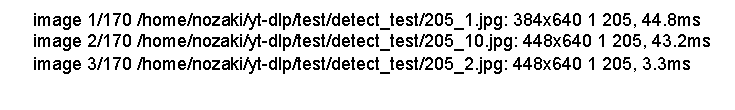
\includegraphics[width=\linewidth]{fig/a.pdf}
	\caption{端末に出力されるもの}\label{output}
\end{figure}

\section{性能の評価}
17種類の各車両の画像を10枚ずつ集めて,テストデータセット作成した.
このテストデータセットと作成したモデルを使って分類または識別を行い,モデルの性能の評価を行う.
\subsection{分類モデルの評価}
%分類モデルの評価を図\ref{CLS}に示す
\begin{figure}	
	\centering
	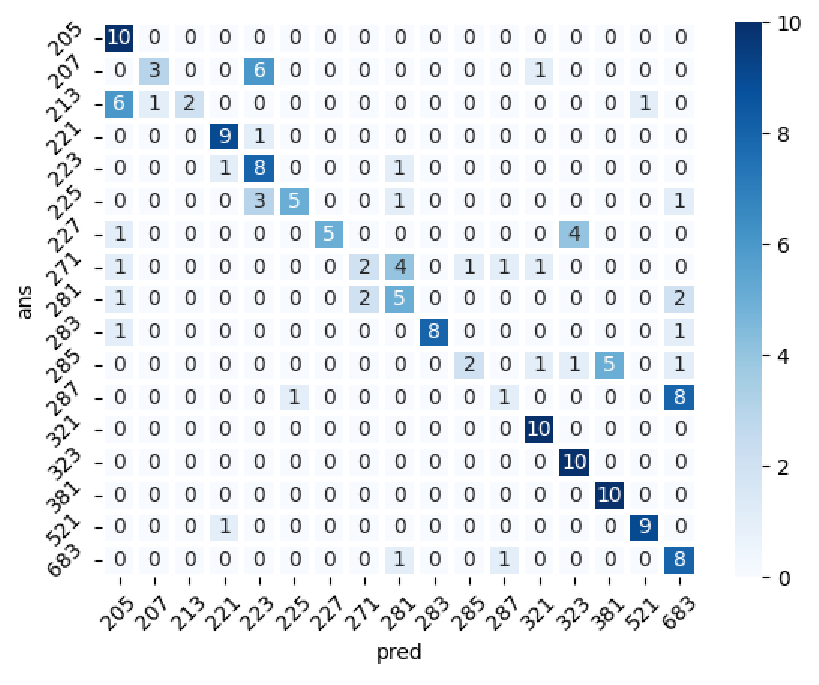
\includegraphics[width=\linewidth]{chap4/fig/classify_results.pdf}
	\caption{分類モデルの評価}
	\label{CLS}
\end{figure}
作成した分類モデルを用いてテストデータセットの分類を行った結果をを図\ref{CLS}に示す.
縦軸が予測した車両タイプ,横軸が正解の車両タイプとするグラフである.

\red{ここに分類結果からわかることを書けば良い?}\\
図\ref{CLS}から,207系と223系,223系と225系,227系と323系,285系と381系,287系と683系の誤分類が多いことがわかる.
%車両の外見は走る路線によって異なり,同じ路線を走る車両は車両タイプが違う場合も外見の色が似ている車両が存在している.
223系,225系は帯の色が,白・青・黄土色の3色で構成されている.
227系は赤色,323系はオレンジ色,
285系と381系は旧国鉄カラー(クリーム色,薄い黄色),
外見が似ている車両タイプは誤分類が多い.
正しく分類できているのは,外見が他の車両と似ていないものばかりだった.



\subsection{識別モデルの評価}
識別失敗数とは間違ったクラスだと判断した数であり,識別不能数とはどのクラスにも当てはまらないと判断した数とする.
識別結果を表\ref{fig:chartdet} に示す.\\
%NaNとは識別成功数または識別失敗数が0のときに,IoUの平均が出せない場合の値である.\\
% TODO: \usepackage{graphicx} required
\begin{figure}[H]
	\centering
	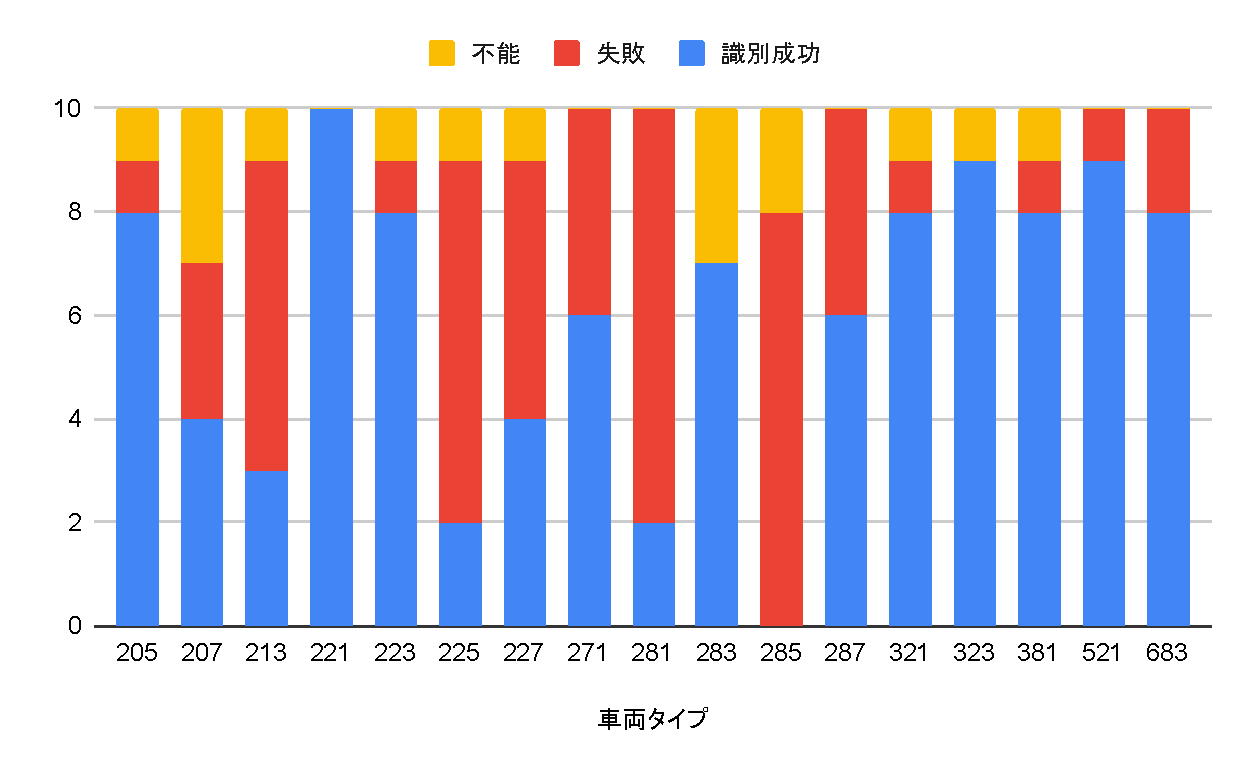
\includegraphics[width=0.7\linewidth]{chap4/fig/chartDET}
	\caption[識別結果]{識別結果}
	\label{fig:chartdet}
\end{figure}


テストデータセットの各画像を識別して7枚以上識別に成功した車両タイプは,205系,221系,223系,283系,321系,323系,381系,521系,683系の9種類だった.
5枚以上識別に失敗している車両タイプは213系,225系,227系,281系,285系の5種類だった.

